
\documentclass{article}
\usepackage{amsmath,float,graphicx,color}
\title{Layered relevance propagation}
\begin{document}
	\maketitle
	\section{Introduction}
	\subsection*{Assumption}
	Before getting started, lets assume the following set up:\\
	A neural network is defined as a function $f(x)$ which has multiple layers and each layer has a set of neurons. These neurons do some element wise computations on pixels(other neurons depending on the complexity of the neural network) which is $x$ followed by non linear activation functions. The final output is represented as $x_{f}$.  Now, the input to neural network is an image of $p$ pixels. This is represented as $\{x_{p}\}$. \\
	 
	There are two main techniques for analyzing neural network prediction.
	\subsection{Sensitivity}
		It  measures the local effect of the neurons for the given output. It is discrete and shows how much impact a neuron makes in deciding the output. 
		\begin{align*}
			\Sigma_{p} (\frac{\delta f}{\delta x_{p}})^2 = \lvert \lvert \Delta_{x} f(x) \rvert \rvert^2
		\end{align*}
	\subsection{Decomposition}
		It measures the global effect for the given ouput. It is contiuous.
		\begin{align*}
			\Sigma_{p} [f(x)]_{p} = f(x)
		\end{align*}
	
	In this blog, we will look into the decomposition analysis of neural networks. 
	\section{Deep Taylor decomposition method}
	
	\subsection{Taylor decomposition}
	A decomposition method based on taylor expansion of a differentiable function $f(x)$ at a root point $\tilde{x}$. The $\tilde{x}$ is chosen such that $f(\tilde{x}) = 0$. The first order taylor expansion is given by:
	\begin{align}
		f(x) &= \left(f(\tilde{x}) + \frac{\delta f}{\delta x} \rvert_{x=\tilde{x}} \right)^{T}. (x - \tilde{x}) + \varepsilon \nonumber  \\
		& \text{In relevance to neural network,}  \nonumber \\
		&= 0+\sum_{p} \frac{\delta f}{\delta x} \rvert_{x = \tilde{x}}. (x_p - \tilde{x}_p) + \varepsilon 
	\end{align}
	The sum was over all pixels $p$ in the image and the ${\tilde{x}_p}$ are the pixel values for root point. The terms inside the sum $\sum_p$ are the relevances assigned to pixels. Therefore, relevance is defined as :
	\begin{align}
		R_p(x) = \frac{\delta f}{\delta x} \rvert_{x = \tilde{x}}. (x_p - \tilde{x}_p)
	\end{align}
	In large deep networks the root point $\tilde{x}$ is hard to perceive for the data point $x$.  \\
	
	This is addressed by \textbf{Deep Taylor decomposition method} by decomposing the already learned function $f(x)$ into a set a sub functions which applies locally to sub set of pixels directly or on abstracted version of them depending on the layer at which they are located in the network.
	\subsection{Relevance Backpropogation}
	Let $f(x)$ yield an output $x_f$. The output is then decomposed on to the neurons present in the previous layers. So, lets take $x_j$ to be a neuron present at a layer and its relevance to be $R_j$. We need to decompose/redistribute $R_j$ on to the set of neurons in the lower layer which connects it and this set is represented as ${x_i}$. Therefore, the relevance$(R_j)$ in terms of $x_i$ is can be derived by the taylor decomposition method explained above, and we define a root point for this decomposition function as $\{\tilde{x}_i\}^{(j)}$. 
	\begin{align}
		R_j &= \Bigg( 
				\frac{\delta R_j}{\delta \{x_i\}}
				\rvert_{\{\tilde{x_i}\}^{(j)}}
			\Bigg)^T
			. (\{x_i\} - \{ \tilde{x_i}^{(j)}\}) + \varepsilon_j \nonumber \\
		  &= \sum_{i} 
			  \underbrace{\frac{\delta R_j}{\delta \{x_i\}}
			  \rvert_{\{\tilde{x_i}^{(j)}\}}
			  . (\{x_i\} - \{ \tilde{x_i}\}^{(j)})}_{R_{ij}} + \varepsilon_j
	\end{align}
	Now, to determine the total relevance of a neuron $x_i$ you need to sum all the relevances contributing to the neuron $x_i$. 
	\begin{align}
		R_i &= \sum_{j} R_{ij} \nonumber \\
		&= \sum_{j} 
		\frac{\delta R_j}{\delta \{x_i\}}
		\rvert_{\{\tilde{x_i}^{(j)}\}}
		. (\{x_i\} - \{ \tilde{x_i}\}^{(j)}) \label{relavance}
	\end{align}
	We can see that there are two features to be noted from the above equations:
	\begin{itemize}
		\item The relevance is conserved during redistribution.
		\item If the values of all neurons  are positive or equal to zero then according to taylor decomposition, the relevance of the same is also positive.
	\end{itemize}
	
	  We take the relevance of the neuron in upper layer and redistribute it to the neurons connected to the lower layer. Similarly, we compute the relevance of the current neuron by summing up the redistributed relevancies of the upper layer neuron which is connected to it. This process is analogous to brack propagation and hence the term \textbf{relevance back propagation}. The below picture would give you a better understanding.
	  
	\begin{figure}[H]
		\centering
		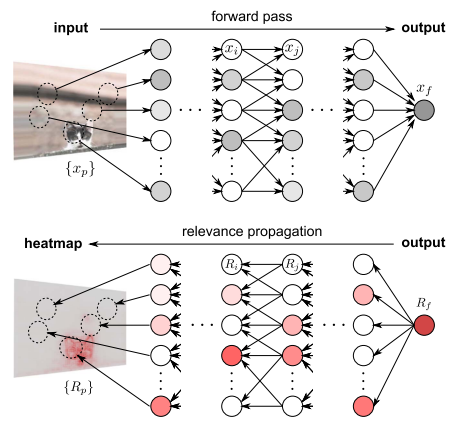
\includegraphics[width=0.65\linewidth]{relevance_bp}
		\caption{Relevance back propagation}
		\label{fig:relevance_bp}
	\end{figure}
	
	\subsection{Choosing a root point}
	It was always said that we would choose a root point in such a way that $f(\tilde{x}) = 0$ but the ways to satisfy that condition was never explained and this section shall discuss that.
	\subsubsection{Unconstrained input space}
	This is the simple and ideal scenario where the input belongs to any real value $X = R^d$. In this case, we can choose the root point $\{ \tilde{x}_i\}^{(j)}$ that is closest in terms of euclidean distance to $\{x_i\}$. Therefore for a positive relevance say $R_j$ the root point in such cases would be intersection of $f(\tilde{x_i}) = 0$ and vector of maximum descent(search direction) is given by $\tilde{x_i}^{(j)} = \{x_i\} + t.\textbf{w}_j$. $\textbf{w}_j$ is the weight parameter connecting the neuron $x_j$.
	\begin{align}
	    \text{Search direction is defined as,} \nonumber \\ \label{search}
		\tilde{x_i}^{(j)} = \{x_i\} + t.\textbf{w}_j  \\
		\text{According to root point definiton,}  \nonumber \\
		f(\tilde{x_i}) = 0   \nonumber \\
		\sum_{i} \tilde{x_i}^{(j)}.w_{ij} + b_j = 0  \label{rt_pt} \\
		\text{Substituting eq (\ref{search}) in  (\ref{rt_pt})}  \nonumber \\
		t = \frac{-1}{\sum_{i} w_{ij}^{2}} . \sum_{i} w_{ij} +b_{j} \nonumber \\
		\text{Injecting it back to eq (\ref{search})} \nonumber \\
		\{\tilde{x_i} \}^{(j)} = \{x_i -  \frac{w_{ij}}{\sum_{i} w_{ij}^{2}} . \sum_{i} w_{ij} +b_{j}  \} \label{rp_val} \\ 
		\text{Therefore substituting (\ref{rp_val}) in equation (\ref{relavance}) and simplifying it,  } \nonumber \\
		R_i = \sum_j (\frac{w_{ij}^{2}}{\sum_{i'} w_{i'j}^2}) R_j  \\
		\textbf{This is the redistributed relevance} \nonumber		
	\end{align}
	\subsubsection{Constrained input space}
	When the input domain $X \subset R^d$ then the nearest root might not be in the same set, hence we restrict our search space according to our feature space domain. Multiple cases of such a setting are explained below.
	\subsubsection*{Application of Rectified Linear Units}
	For ReLU, the search domain is restricted to only the positive part of $w_{ij}$ and hence the redistributed relevance is given by:
	\begin{align}
		R_i = \sum_{j} \frac{z_{ij}^{+}}{\sum_{i'}z_{i'j}^{+}} R_j
		%\
	\end{align}
	where $z_{ij}^{+} = x_iw_{ij}^{+}$ and $w_{ij}^{+}$ denotes positive part of $w_{ij}$.
	\subsubsection*{Application for Images as inputs}
	Similarly in the case of image classification tasks, we would consider only those feature spaces that fall under the domain of admissible pixel values in each dimension. The input space can be written as,
	\begin{align}
		B = \{ \{ x_i\}: \forall_{i=1}^{d} l_i \leq x_i \leq h_i \} \nonumber 
	\end{align}
	where the input has \textit{d} dimensions and $l_i \leq 0$ \& $h_i \geq 0$ are the smallest and largest admissible pixel for each dimension. Then, the redistributed relevance is: 
	
	\begin{align}
		R_i = \sum_j \frac{z_{ij} - l_i w_{ij}^{+} - h_i w_{ij}^{-} }{\sum_{i'}z_{i'j} - l_i w_{i'j}^{+} - h_i w_{i'j}^{-} }
	\end{align}
	

	
	

\end{document}